\documentclass[12pt]{article}

% Pacotes básicos
\usepackage[brazil]{babel}
\usepackage[utf8]{inputenc}
\usepackage[T1]{fontenc}
\usepackage{graphicx}  
\usepackage{booktabs}   
\usepackage{float}      
\usepackage{geometry}
\usepackage{setspace}
\usepackage{listings}
\usepackage{xcolor}
\usepackage[hidelinks]{hyperref}
\usepackage{csvsimple}

\lstset{
    basicstyle=\ttfamily\scriptsize,
    frame=single,
    breaklines=true,
    aboveskip=6pt,
    belowskip=6pt,
    inputencoding=utf8,
    extendedchars=true,
    literate=
      {á}{{\'a}}1
      {à}{{\`a}}1
      {ã}{{\~a}}1
      {â}{{\^a}}1
      {é}{{\'e}}1
      {ê}{{\^e}}1
      {í}{{\'i}}1
      {ó}{{\'o}}1
      {ô}{{\^o}}1
      {õ}{{\~o}}1
      {ú}{{\'u}}1
      {ç}{{\c{c}}}1
      {Á}{{\'A}}1
      {À}{{\`A}}1
      {Ã}{{\~A}}1
      {Â}{{\^A}}1
      {É}{{\'E}}1
      {Ê}{{\^E}}1
      {Í}{{\'I}}1
      {Ó}{{\'O}}1
      {Ô}{{\^O}}1
      {Õ}{{\~O}}1
      {Ú}{{\'U}}1
      {Ç}{{\c{C}}}1
}


\geometry{margin=2.5cm}
\onehalfspacing

% Informações do artigo
\title{Comparação de Algoritmos de Ordenação}
\author{
Pedro Alonso de Aguiar Fernandes \\
Talles Vieira Ferreira Bazani Gonçalves \\
Universidade Federal do Espírito Santo
}
\date{2025}

\begin{document}

\maketitle

% ---------------- RESUMO ----------------
\begin{abstract}
Este trabalho apresenta uma análise comparativa de algoritmos de ordenação, avaliando
seu desempenho a partir de métricas como o número de comparações, o número de trocas e
o tempo de execução. Os experimentos foram realizados utilizando diferentes tipos de entrada
(aleatória, crescente e decrescente) e tamanhos de vetores, com o objetivo de identificar as
vantagens e desvantagens de cada algoritmo em diferentes cenários.
\end{abstract}

\newpage

\setcounter{tocdepth}{2}
\tableofcontents

\newpage

% ---------------- INTRODUÇÃO ----------------
\section{Introdução}

O crescente volume de dados manipulados por sistemas computacionais torna essencial
a utilização de algoritmos eficientes para organização e processamento da informação.
Nesse contexto, os algoritmos de ordenação desempenham um papel fundamental, sendo
amplamente utilizados como etapa inicial de diversos problemas computacionais.

O estudo e a análise experimental desses algoritmos permitem compreender não apenas
sua complexidade teórica, mas também seu comportamento prático diante de diferentes
tipos de entrada. Dependendo da organização inicial dos dados, um mesmo algoritmo pode
apresentar desempenhos significativamente distintos.

Dessa forma, este trabalho tem como objetivo comparar experimentalmente diferentes
algoritmos de ordenação, analisando métricas de desempenho como tempo de execução,
número de comparações e número de trocas. Os testes foram realizados com vetores de
diferentes tamanhos e ordens iniciais, possibilitando uma análise abrangente do
comportamento dos algoritmos estudados.

% ---------------- METODOLOGIA ----------------
\section{Metodologia}

Para a realização dos experimentos, todos os algoritmos de ordenação foram
implementados na linguagem de programação C. Os testes foram conduzidos utilizando
vetores de números inteiros gerados automaticamente, de acordo com três configurações
distintas: ordem aleatória, ordem crescente e ordem decrescente.

Os tamanhos dos vetores utilizados nos experimentos foram de 10.000, 100.000 e
500.000 elementos. Para cada combinação
de algoritmo, tipo de entrada e tamanho de vetor, foram coletados dados referentes ao
tempo de execução, número de comparações e número de trocas realizadas durante o
processo de ordenação.

Os experimentos foram executados em um notebook com as seguintes configurações de
hardware e software:

\begin{itemize}
    \item Fabricante: Acer;
    \item Modelo: Aspire 5 A515-45;
    \item Processador: AMD Ryzen 7 5700U;
    \item Memória RAM: 16 GB;
    \item Sistema Operacional: Microsoft Windows 11 Pro (64 bits).
\end{itemize}

Os resultados obtidos foram organizados em tabelas e gráficos, permitindo uma análise
comparativa entre os algoritmos. A partir desses dados, foi realizada uma discussão
crítica sobre o desempenho observado em cada cenário experimental.

% ---------------- ALGORITMOS ----------------
\section{Algoritmos de Ordenação}

Algoritmos de ordenação são métodos utilizados para organizar um conjunto de dados
segundo um critério específico, normalmente em ordem crescente ou decrescente. Eles
desempenham um papel fundamental em diversas aplicações computacionais, pois influenciam
diretamente a eficiência de operações como busca, análise e processamento de informações.

Neste trabalho, são apresentados e analisados diferentes algoritmos de ordenação,
abrangendo desde métodos simples, baseados em comparações diretas, até algoritmos mais
eficientes, que apresentam melhor desempenho para grandes volumes de dados.

\subsection{Bolha}

O algoritmo Bolha funciona percorrendo repetidamente o vetor e comparando elementos adjacentes, trocando-os de posição sempre que o elemento da esquerda é maior que o da direita. A cada passagem completa pelo vetor, o maior valor ainda não ordenado é deslocado para o final, reduzindo gradualmente a parte do vetor que precisa ser analisada, até que todos os elementos estejam em ordem crescente \cite{cormen2009}.

% Código do algoritmo Bolha
\begin{lstlisting}
void bolha(int* vetor, int tamanho, Registro* registro){
    int aux;
    for(int i = tamanho - 1; i >= 1; i--){
        for(int j = 0; j < i; j++){	  
            registro->comparacoes++; // Contabiliza compração
            if (vetor[j] > vetor[j + 1]) {
                aux = vetor[j];
                vetor[j] = vetor[j + 1];
                vetor[j + 1] = aux;
                registro->trocas++; // Contabiliza troca
            }
        }
    }
}
\end{lstlisting}

\newpage

\subsection{Bolha com Critério de Parada}

O algoritmo Bolha com Critério de Parada funciona de forma semelhante ao algoritmo Bolha tradicional, comparando elementos adjacentes do vetor e realizando trocas sempre que o elemento da esquerda é maior que o da direita. A diferença está no uso de uma variável de controle que indica se houve alguma troca durante uma passagem completa pelo vetor, caso nenhuma troca ocorra, o algoritmo é interrompido, pois isso indica que o vetor já está ordenado e não é necessário continuar as comparações \cite{cormen2009}.

% Código do algoritmo Bolha com Critério de Parada
\begin{lstlisting}
void bolhaComParada(int* vetor, int tamanho, Registro* registro){
    int aux;
    int trocou;
    for(int i = tamanho - 1; i >= 1; i--){
        trocou = 0;
        for(int j = 0; j < i; j++){
            registro->comparacoes++; // Contabiliza comparação
            if(vetor[j] > vetor[j + 1]){
                aux = vetor[j];
                vetor[j] = vetor[j + 1];
                vetor[j + 1] = aux;
                registro->trocas++; // Contabiliza troca
                trocou = 1; // Marcou que houve troca
            }
        }
        // Critério de parada
        if(trocou == 0){
            break;
        }
    }
}
\end{lstlisting}

\subsection{Inserção Direta}

O algoritmo Inserção Direta funciona percorrendo o vetor a partir do segundo elemento, considerando que o primeiro já se encontra ordenado, e inserindo cada novo valor na posição correta entre os elementos analisados à sua esquerda. Em cada passo, o elemento atual é armazenado temporariamente e comparado com os valores anteriores, que são deslocados uma posição para a direita sempre que forem maiores do que ele. Esse processo continua até que seja encontrada a posição adequada para a inserção, garantindo que, ao final de cada iteração, o trecho inicial do vetor permaneça ordenado, enquanto o algoritmo avança progressivamente até ordenar todo o conjunto de dados \cite{ziviani2012}.

\newpage

% Código do algoritmo de Inserção Direta 
\begin{lstlisting}
void insercaoDireta(int* vetor, int tamanho, Registro* registro){
    int aux;
    int j;
    for(int i = 1; i < tamanho; i++){
        aux = vetor[i];
        j = i - 1;
        while(j >= 0){
            registro->comparacoes++; // Contabiliza comparação
            if(aux < vetor[j]){
                vetor[j + 1] = vetor[j];
                registro->trocas++; // Contabiliza troca
                j--;
            } 
            else {
                break;
            }		
        }
        if(j != i - 1){
            vetor[j + 1] = aux; // Essa troca já foi contabilizada 
                                // dentro do if do while acima
        }
    }
}
\end{lstlisting}

\subsection{Inserção Binária}

O algoritmo Inserção Binária funciona de forma semelhante à Inserção Direta, mantendo sempre a parte inicial do vetor ordenada, porém utiliza uma busca binária para determinar a posição correta onde o elemento atual deve ser inserido. A cada iteração, o elemento selecionado é comparado com os valores do trecho já ordenado, reduzindo gradualmente o intervalo de busca até localizar a posição adequada. Após essa posição ser encontrada, os elementos maiores são deslocados uma posição para a direita, abrindo espaço para a inserção do valor sem comprometer a ordenação existente no vetor, garantindo que a sequência inicial permaneça ordenada ao final de cada passo do algoritmo \cite{cormen2009}.

\newpage

% Código do algoritmo de Inserção Binária
\begin{lstlisting}
void insercaoBinaria(int* vetor, int tamanho, Registro* registro){
    int aux;
    int esq, dir, meio;
    for(int i = 1; i < tamanho; i++){
        aux = vetor[i];
        esq = 0;
        dir = i;
        // Busca binária da posição correta
        while(esq < dir){
            meio = (esq + dir) / 2;	
            registro->comparacoes++; // Contabiliza comparação
            if(vetor[meio] <= aux){
                esq = meio + 1;
            } 
            else {
                dir = meio;
            }	
        }
        // Deslocando elementos
        for(int j = i; j > esq; j--){
            vetor[j] = vetor[j - 1];
            registro->trocas++; // Contabiliza troca
        }
        vetor[esq] = aux; // Essa troca já foi contabilizada no for acima	  
    }
}
\end{lstlisting}

\subsection{Inserção Ternária}

O algoritmo Inserção Ternária organiza o vetor mantendo sempre a parte inicial ordenada e inserindo cada novo elemento na posição correta. Para isso, a cada iteração, o elemento atual é armazenado temporariamente e o trecho já ordenado é analisado por meio de uma busca ternária, na qual o intervalo é dividido em três partes utilizando dois pontos intermediários. Com base nas comparações realizadas, o algoritmo determina em qual desses subintervalos o elemento deve ser inserido, reduzindo gradualmente a região de busca até encontrar a posição adequada. Após essa definição, os elementos maiores são deslocados uma posição para a direita, permitindo a inserção do valor sem quebrar a ordenação existente no vetor \cite{ziviani2012}.

\newpage

% Código do algoritmo de Inserção Ternária
\begin{lstlisting}
void insercaoTernaria(int* vetor, int tamanho, Registro* registro){
    int aux;
    int esq, dir;
    int div1, div2;
    for(int i = 1; i < tamanho; i++){
        aux = vetor[i];
        esq = 0;
        dir = i;
        // Busca ternária da posição correta
        while(esq < dir){
            div1 = esq + (dir - esq) / 3;
            div2 = esq + 2 * (dir - esq) / 3;
            registro->comparacoes++; // Contabiliza comparação
            if(aux < vetor[div1]){
                dir = div1;
            }
            else{
                registro->comparacoes++; // Contabiliza comparação
                if(aux > vetor[div2]){
                    esq = div2 + 1;
                }
                else{
                    esq = div1 + 1;
                    dir = div2;
                }
			}
        }
        // Deslocando elementos
        for(int j = i; j > esq; j--){
            vetor[j] = vetor[j - 1];
            registro->trocas++; // Contabiliza troca
        }
        vetor[esq] = aux; // Essa troca já foi contabilizada no for acima
    }
}
\end{lstlisting}

\subsection{Shell Sort}

O algoritmo Shell Sort funciona como uma generalização da Inserção Direta, utilizando comparações entre elementos que estão a uma certa distância definida por um intervalo, denominado gap. Inicialmente, é escolhido um valor de gap maior que um, e o vetor é percorrido realizando inserções entre elementos separados por esse intervalo, organizando subvetores formados por essas posições. À medida que o gap é reduzido, o algoritmo repete o processo até que o intervalo seja igual a um, momento em que o vetor já se encontra parcialmente ordenado, permitindo que a ordenação final ocorra de forma semelhante à Inserção Direta \cite{ziviani2012}.

\newpage

% Código do algoritmo Shell Sort
\begin{lstlisting}
void shellSort(int* vetor, int tamanho, Registro* registro){
    int gap = 1; // Intervalo 
    int aux;
    int j;
    // Geração do intervalo
    while(gap < tamanho){
        gap = 3 * gap + 1;
    }
    while(gap > 1){
        gap = gap / 3;
        for(int i = gap; i < tamanho; i++){
            aux = vetor[i];
            j = i - gap;
            while(j >= 0){		
                registro->comparacoes++; // Contabiliza comparação
                if(aux < vetor[j]){
                    vetor[j + gap] = vetor[j];
                    registro->trocas++; // Contabiliza troca
                    j = j - gap;
                }
                else {
                    break;
                }	
            }
            vetor[j + gap] = aux;   // Essa troca já foi contabilizada 
                                    // dentro do if do while acima	
        }
    }
}
\end{lstlisting}

\subsection{Selection Sort}

O algoritmo Selection Sort funciona organizando o vetor por meio da seleção repetida do menor elemento da parte ainda não ordenada. Em cada iteração, o algoritmo percorre o trecho restante do vetor para identificar o menor valor e, ao final dessa busca, realiza uma troca colocando esse elemento na posição correta, no início da parte não ordenada. Esse processo se repete até que todos os elementos tenham sido posicionados, resultando em um vetor ordenado de forma crescente \cite{ziviani2012}.

\newpage

% Código do algoritmo Selection Sort
\begin{lstlisting}
void selectionSort(int* vetor, int tamanho, Registro* registro){	
    registro->comparacoes = 0; // Comparações
    registro->trocas = 0; // Trocas 
    for(int i = 0; i < (tamanho - 1); i++){
        int indice_menor = i;
        for(int j = i + 1; j < tamanho; j++){
            registro->comparacoes++; // Contabiliza comparação
            if(vetor[j] < vetor[indice_menor]){
                indice_menor = j;
            }
        }
        registro->comparacoes++; // Contabiliza comparação
        if(indice_menor != i){
            int aux = vetor[i];
            vetor[i] = vetor[indice_menor];
            vetor[indice_menor] = aux;
            registro->trocas++; // Cotabiliza troca
        }
    }
}
\end{lstlisting}

\subsection{Heap Sort}

O algoritmo Heap Sort organiza os elementos do vetor utilizando uma estrutura de dados do tipo árvore binária, conhecida como heap, que pode ser representada diretamente em um array. Nesse método, o vetor é interpretado como uma árvore binária completa, em que cada posição corresponde a um nó e seus filhos são definidos por índices específicos do vetor. A organização segue a propriedade de heap máximo, na qual o valor armazenado no nó pai é sempre maior ou igual aos valores de seus filhos, garantindo que o maior elemento esteja sempre na raiz da árvore. Inicialmente, o algoritmo ajusta o vetor para que todas as subárvores satisfaçam essa propriedade e, em seguida, o maior elemento é removido da raiz e colocado na última posição do vetor. Esse processo é repetido, reduzindo o tamanho da árvore e reorganizando a estrutura até que todos os elementos estejam ordenados \cite{cormen2009}.

\newpage

% Código do algoritmo Heap Sort
\begin{lstlisting}
void heapify(int* vetor, int tamanho, int raiz, Registro* registro){
    int maior = raiz; // Supõe que a raiz é o maior número
    int esquerda = (2 * raiz) + 1;  // Conta para lidar um array como uma árvore binária. 
                                    //Isso pega o filho à esquerda
    int direita = (2 * raiz) + 2;   // Conta para lidar um array como uma árvore binária. 
                                    // Isso pega o filho à direita
    // Verifica se existe um filho à esquerda, 
    // e verifica se o filho da esquerda é maior do que a raiz
    registro->comparacoes++; // Contabiliza comparação
    if(esquerda < tamanho && vetor[esquerda] > vetor[maior]){
        maior = esquerda;
    }
    // Verifica se existe filho à direita, 
    // e verifica se o filho da direita é maior do que o maior número conhecido 
    // até agora (Seja a raiz, ou o filho da esquerda)
    registro->comparacoes++; // Contabiliza comparação
    if(direita < tamanho && vetor[direita] > vetor[maior]){
        maior = direita;
    }
    // Se o maior valor não for a raiz, troca de posição com a raiz e
    // heapifica (deixar em max heap) a "nova subárvore"
    registro->comparacoes++; // Contabiliza comparação
    if(maior != raiz){
        int aux = vetor[raiz];
        vetor[raiz] = vetor[maior];
        vetor[maior] = aux;
        registro->trocas++; //Contabiliza troca
        // Heapifica a "nova subárvore" recursivamente
        heapify(vetor, tamanho, maior, registro);
    }
}
\end{lstlisting}

\begin{lstlisting}
void heapSort(int* vetor, int tamanho, Registro* registro){
    // Deixa toda a árvore em max heap, chamando o heapify em todo ramo que possui filho
    for(int i = (tamanho / 2) - 1; i >= 0; i--)
        heapify(vetor, tamanho, i, registro);
    // Pega o maior elemento da árvore (raiz), 
    // coloca por último no vetor e subtrai 1 do tamanho da árvore.
    // Assim sucessivamente até o vetor estar ordenado
    for(int i = tamanho - 1; i >= 0; i--){
        int aux = vetor[i];
        vetor[i] = vetor[0];
        vetor[0] = aux;
        registro->trocas++; // Contabiliza troca
        // Deixa a nova árvore em max heap
        heapify(vetor, i, 0, registro);
    }
}
\end{lstlisting}

\newpage

\subsection{Quick Sort Centro}

O algoritmo Quick Sort com pivô no centro funciona escolhendo o elemento localizado na posição central do vetor como referência para a ordenação. A partir desse pivô, o vetor é reorganizado de modo que os elementos menores fiquem à esquerda e os maiores à direita, formando dois subvetores. Esse processo de separação divide o problema em partes menores, que são tratadas de forma recursiva até que todos os elementos estejam posicionados corretamente, resultando na ordenação completa do vetor \cite{cormen2009}.

\subsubsection{Quick Sort Centro (Lomuto)}

O algoritmo Quick Sort com pivô no centro utilizando o método de partição de Lomuto funciona escolhendo como pivô o elemento localizado na posição central do vetor, que é inicialmente movido para o final para facilitar o processo de partição. Em seguida, o algoritmo percorre o vetor do início até a posição anterior ao pivô, comparando cada elemento com o valor do pivô e reorganizando os dados de modo que todos os elementos menores ou iguais a ele sejam colocados à esquerda. Ao final dessa varredura, o pivô é reposicionado em sua posição correta, separando o vetor em duas partes, que são ordenadas recursivamente pelo mesmo procedimento até que todo o vetor esteja ordenado \cite{sedgewick2011}.

% Código do algoritmo Quick Sort Centro (Lomuto)
\begin{lstlisting}
int particaoCentroLomuto(int* vetor, int inicio, int fim, Registro* registro){
    int centro = inicio + (fim - inicio) / 2;
    int pivo = vetor[centro];
    int posicaoPivo = inicio;
    // Move o pivô para o último elemento do vetor
    int aux = vetor[fim];
    vetor[fim] = vetor[centro];
    vetor[centro] = aux;
    registro->trocas++; // Contabiliza troca
    for(int j = inicio; j < fim; j++){	
        registro->comparacoes++; // Contabiliza comparação
        if(vetor[j] <= pivo){
            int aux = vetor[posicaoPivo];
            vetor[posicaoPivo] = vetor[j];
            vetor[j] = aux;
            registro->trocas++; // Contabiliza troca
            posicaoPivo++;
        }
    }
    aux = vetor[posicaoPivo];
    vetor[posicaoPivo] = vetor[fim];
    vetor[fim] = aux;
    registro->trocas++; // Contabiliza troca
    return posicaoPivo;
}
\end{lstlisting}

\newpage

\begin{lstlisting}
void quickSortCentroLomuto(int* vetor, int inicio, int fim, Registro* registro){
    if(inicio < fim){
        // Escolhe um pivô e deixa número menores à esquerda e maiores à direita
        int posicaoPivo = particaoCentroLomuto(vetor, inicio, fim, registro); 
        // Ordena o lado esquerdo do pivô
        quickSortCentroLomuto(vetor, inicio, posicaoPivo - 1, registro); 
        // Ordena o lado direito do pivô
        quickSortCentroLomuto(vetor, posicaoPivo + 1, fim, registro); 
    }
}
\end{lstlisting}

\subsubsection{Quick Sort Centro (Hoare)}

O algoritmo Quick Sort com pivô no centro pelo método de Hoare escolhe o elemento central como pivô e utiliza dois ponteiros que percorrem o vetor a partir das extremidades, comparando os valores com o pivô. Sempre que um valor maior que o pivô é encontrado à esquerda e um menor à direita, esses elementos são trocados, e o processo continua até que os ponteiros se cruzem. Ao final, o vetor é dividido em duas partes em torno do pivô, que são ordenadas recursivamente pelo mesmo procedimento \cite{cormen2009}.

% Código do algoritmo Quick Sort Centro (Hoare)
\begin{lstlisting}
int particaoCentroHoare(int* vetor, int inicio, int fim, Registro* registro){
    // Escolhe o pivô no centro
    int centro = inicio + (fim - inicio) / 2;
    int pivo = vetor[centro];
    int i = inicio - 1;
    int j = fim + 1;
    while (1) {
        // Move o ponteiro i para a direita enquanto o valor for menor que o pivô
        do {
            i++;
            registro->comparacoes++; // Contabiliza comparação
        } 
        while (vetor[i] < pivo);
        // Move o ponteiro j para a esquerda enquanto o valor for maior que o pivô
        do {
            j--;
            registro->comparacoes++; // Contabiliza comparação
        } 
        while (vetor[j] > pivo);
        // Se os ponteiros se cruzarem, a partição acabou
        if (i >= j) {
            return j;
        }
        // Se encontrou um valor maior à esquerda e um menor à direita, troca-os
        int aux = vetor[j];
        vetor[j] = vetor[i];
        vetor[i] = aux;
        registro->trocas++; // Contabiliza troca
    }
}
\end{lstlisting}

\begin{lstlisting}
void quickSortCentroHoare(int* vetor, int inicio, int fim, Registro* registro){
    if(inicio < fim){
        // Escolhe um pivô e deixa número menores ou iguais à esquerda e maiores à direita
        int p = particaoCentroHoare(vetor, inicio, fim, registro);		
        // Até o indice p, os números do vetor são menores ou iguais ao pivô. 
        // Depois dele, os números são maiores que o pivô
        // Ordena os número menores ou iguais ao pivô
        quickSortCentroHoare(vetor, inicio, p, registro);		
        // Ordena os número maiores que o pivô
        quickSortCentroHoare(vetor, p + 1, fim, registro);	
    }
}
\end{lstlisting}

\subsection{Quick Sort Fim}

O Quick Sort com pivô no fim funciona escolhendo sempre o último elemento do trecho do vetor como pivô e reorganizando os demais valores em relação a ele. O algoritmo percorre o vetor do início até a posição anterior ao pivô, comparando cada elemento com esse valor final; sempre que encontra um elemento menor ou igual ao pivô, ele é trocado para a posição mais à esquerda ainda disponível, mantendo os menores à esquerda e os maiores à direita. Ao final desse percurso, o pivô é colocado exatamente na posição correta, de forma que todos os elementos à sua esquerda são menores ou iguais e todos à direita são maiores. Em seguida, o mesmo processo é aplicado recursivamente às duas partes do vetor formadas em torno do pivô, repetindo essa ideia até que todo o vetor esteja ordenado \cite{cormen2009}.

% Código do algoritmo Quick Sort Fim
\begin{lstlisting}
int particaoFim(int* vetor, int inicio, int fim, Registro* registro){
    int pivo = vetor[fim];
    int posicaoPivo = inicio;
    for(int j = inicio; j < fim; j++){
        registro->comparacoes++; // Contabiliza comparação
        if(vetor[j] <= pivo){
            int aux = vetor[posicaoPivo];
            vetor[posicaoPivo] = vetor[j];
            vetor[j] = aux;
            registro->trocas++; // Contabiliza troca
            posicaoPivo++;
        }
    }  
    int aux = vetor[posicaoPivo];
    vetor[posicaoPivo] = vetor[fim];
    vetor[fim] = aux;
    registro->trocas++; // Contabiliza troca
    return posicaoPivo;
}
\end{lstlisting}

\newpage

\begin{lstlisting}
void quickSortFim(int* vetor, int inicio, int fim, Registro* registro){
    /* O código abaixo funciona, porém quando quando o vetor é crescente de 500 mil elementos, a recursão dele exige muita memória e acaba dando erro de segmentação
    if(inicio < fim){
        // Escolhe um pivô e deixa número menores à esquerda e maiores à direita
        int posicaoPivo = particaoFim(vetor, inicio, fim, registro);	
        // Ordena o lado esquerdo do pivô
        quickSortFim(vetor, inicio, posicaoPivo - 1, registro);	
        // Ordena o lado direito do pivô
        quickSortFim(vetor, posicaoPivo + 1, fim, registro);		
    } */
    while (inicio < fim) {
        int p = particaoFim(vetor, inicio, fim, registro);
        // Otimização: Escolhe sempre o lado MENOR para a recursão
        if (p - inicio < fim - p) {
            quickSortFim(vetor, inicio, p - 1, registro);
            inicio = p + 1; // Transforma a chamada da direita em um loop (iteração)
        } 
        else {
            quickSortFim(vetor, p + 1, fim, registro);
            fim = p - 1; // Transforma a chamada da esquerda em um loop (iteração)
        }
    }
}
\end{lstlisting}

\subsection{Quick Sort Mediana}

O quick sort mediana funciona escolhendo o pivô a partir da mediana entre três elementos do vetor: o primeiro, o elemento central e o último. Inicialmente, esses três valores são comparados e trocados entre si até ficarem ordenados, garantindo que o valor intermediário entre eles fique na posição central e seja usado como pivô. Em seguida, dois índices percorrem o vetor a partir das extremidades, avançando enquanto encontram valores menores ou maiores que o pivô, e realizando trocas quando elementos fora da posição correta são encontrados, de modo que os valores menores ou iguais ao pivô fiquem à esquerda e os maiores fiquem à direita. Quando os índices se cruzam, a partição termina e o algoritmo é chamado recursivamente para as duas partes do vetor, repetindo o mesmo procedimento até que todo o vetor esteja ordenado \cite{cormen2009}.

% Código do algoritmo Quick Sort Mediana
\begin{lstlisting}
int particaoMediana(int* vetor, int inicio, int fim, Registro* registro){
    int meio = inicio + (fim - inicio) / 2;
    // Ordena o primeiro, o do meio e o último elemento. Ao final, a mediana estará no meio.
    registro->comparacoes++; // Contabiliza comparação
    if(vetor[inicio] > vetor[meio]){
        int aux = vetor[meio];
        vetor[meio] = vetor[inicio];
        vetor[inicio] = aux;
        registro->trocas++; // Contabiliza troca
    }
    registro->comparacoes++; // Contabiliza comparação
    if(vetor[inicio] > vetor[fim]){
        int aux = vetor[fim];
        vetor[fim] = vetor[inicio];
        vetor[inicio] = aux;
        registro->trocas++; // Contabiliza troca
    }
    registro->comparacoes++; // Contabiliza comparação
    if(vetor[meio] > vetor[fim]){
        int aux = vetor[fim];
        vetor[fim] = vetor[meio];
        vetor[meio] = aux;
        registro->trocas++; // Contabiliza troca
    }
    // A mediana agora está no meio
    int pivo = vetor[meio];
    int i = inicio - 1;
    int j = fim + 1;
    while (1) {
        // Move o ponteiro i para a direita enquanto o valor for menor que o pivô
        do {
            i++;
            registro->comparacoes++; // Contabiliza comparação
        } while (vetor[i] < pivo);
        // Move o ponteiro j para a esquerda enquanto o valor for maior que o pivô
        do {
            j--;
            registro->comparacoes++; // Contabiliza comparação
        } while (vetor[j] > pivo);
        // Se os ponteiros se cruzarem, a partição acabou
        if (i >= j) {
            return j;
        } 
        // Se encontrou um valor maior à esquerda e um menor à direita, troca-os
        int aux = vetor[j];
        vetor[j] = vetor[i];
        vetor[i] = aux;
        registro->trocas++; // Contabiliza troca
    }
}
\end{lstlisting}

\begin{lstlisting}
void quickSortMediana(int* vetor, int inicio, int fim, Registro* registro){
    if(inicio < fim){
        // Escolhe um pivô e deixa número menores ou iguais à esquerda e maiores à direita
        int p = particaoMediana(vetor, inicio, fim, registro); 
        // Até o indice p, os números do vetor são menores ou iguais ao pivô,
        // depois dele, os números são maiores que o pivô.
        // Ordena os número menores ou iguais ao pivô
        quickSortMediana(vetor, inicio, p, registro); 
        // Ordena os número maiores que o pivô
        quickSortMediana(vetor, p + 1, fim, registro); 
    }
}
\end{lstlisting}

\subsection{Merge Sort}

O Merge Sort funciona dividindo o vetor original em duas partes menores de forma recursiva, até que cada parte tenha apenas um elemento, pois um vetor com um único elemento já está ordenado. Em seguida, essas partes são combinadas novamente por meio do processo de intercalação, no qual dois vetores já ordenados são comparados elemento a elemento e reorganizados em um único vetor também ordenado, copiando sempre o menor valor disponível para o vetor principal. Esse processo de divisão e intercalação continua até que todas as partes tenham sido reunidas, resultando no vetor completamente ordenado \cite{cormen2009}.

% Código do algoritmo Merge Sort
\begin{lstlisting}
void merge(int* vetor, int inicio, int meio, int tamanho, Registro* registro){
    // Separa o vetor em dois vetores
    int tam_esquerda = meio - inicio;
    int tam_direita = tamanho - meio;
    int* vetor_esquerda = (int*) malloc(tam_esquerda * sizeof(int));	
    int* vetor_direita = (int*) malloc(tam_direita * sizeof(int));	
    for(int i = 0; i < tam_esquerda; i++){
        vetor_esquerda[i] = vetor[inicio + i];
    }
    for(int i = 0; i < tam_direita; i++){
        vetor_direita[i] = vetor[meio + i];
    }
    // Ordena o vetor principal de acordo com os outros dois vetores
    int topo_esquerda = 0;
    int topo_direita = 0;
    int k = inicio;
    // Enquanto houver elementos nos dois vetores simultâneamente, 
    // eles serão comparados e ordenados no vetor principal
    while (topo_esquerda < tam_esquerda && topo_direita < tam_direita) {
        registro->comparacoes++; // Contabiliza comparação
        if (vetor_esquerda[topo_esquerda] <= vetor_direita[topo_direita]) {
            vetor[k] = vetor_esquerda[topo_esquerda];
            topo_esquerda++;
        } 
        else {
            vetor[k] = vetor_direita[topo_direita];
            topo_direita++;
        }
        k++;
        registro->trocas++; // Contabiliza troca
    }
    // Copia os elementos do vetor em que sobrou elementos
    while (topo_esquerda < tam_esquerda) {
        vetor[k] = vetor_esquerda[topo_esquerda];
        registro->trocas++; // Contabiliza troca
        topo_esquerda++;
        k++;
    }
    while (topo_direita < tam_direita) {
        vetor[k] = vetor_direita[topo_direita];
        registro->trocas++; // Contabiliza troca
        topo_direita++;
        k++;
    }
    free(vetor_esquerda);
    free(vetor_direita);
}
\end{lstlisting}

\begin{lstlisting}
void mergeSort(int* vetor, int inicio, int tamanho, Registro* registro){
    // Divide o vetor em vetores menores (até chegar em um vetor de 1 elemento) 
    // e os reagrupa em um vetor ordenado
    if(tamanho - inicio > 1){
        int meio = inicio + (tamanho - inicio) / 2;
        mergeSort(vetor, inicio, meio, registro);
        mergeSort(vetor, meio, tamanho, registro);
        merge(vetor, inicio, meio, tamanho, registro);
    }
}
\end{lstlisting}

\subsection{Radix Sort}

O algoritmo Radix Sort ordena os elementos do vetor analisando os valores dígito a dígito, começando pelo dígito menos significativo e avançando gradualmente para os mais significativos. Em cada etapa, o algoritmo considera uma casa decimal específica e reorganiza os elementos com base nesse dígito, utilizando um método auxiliar de contagem para agrupar valores que possuem o mesmo algarismo naquela posição. Esse processo é repetido para todas as casas decimais necessárias, até que o maior número do vetor seja completamente analisado. Ao final dessas iterações sucessivas, os elementos ficam ordenados de forma crescente, sem a necessidade de comparações diretas entre pares de valores, pois a ordenação ocorre a partir da distribuição dos dígitos \cite{cormen2009}.

% Código do algoritmo Radix Sort
\begin{lstlisting}
void ordenarPorDigito(int* vetor, int tamanho, int expoente, Registro* registro){
    int* saida = (int*) malloc(tamanho * sizeof(int));
    int count_digito[10] = {0};	// Separa uma posição do vetor para cada algarismo (0 a 9)
    if(saida != NULL){
        // Conta quantos elementos diferentes tem o mesmo algarismo na referida casa decimal
        for(int i = 0; i < tamanho; i++){
            int digito = (vetor[i] / expoente) % 10;
            count_digito[digito]++;
        }
        // Ajusta a posição de cada algarismo de acordo com a sua quantidade
        for(int i = 1; i < 10; i++){
            count_digito[i] += count_digito[i - 1];
        }
        // Cria um vetor já inserindo de forma ordenada
        for(int i = tamanho - 1; i >= 0; i--){
            int digito = (vetor[i] / expoente) % 10;
            saida[count_digito[digito] - 1] = vetor[i];
            count_digito[digito]--;
        }
        // Copia o vetor ordenado para o vetor principal
        for(int i = 0; i < tamanho; i++){
            vetor[i] = saida[i];
            registro->trocas++; // Contabiliza troca
        }
        free(saida);
    }
    else
        printf("Erro ao alocar memória para o vetor \"saida\"!\n");
}
\end{lstlisting}

\begin{lstlisting}
void radixSort(int* vetor, int tamanho, Registro* registro){
    int maior = vetor[0];
    for(int i = 1; i < tamanho; i++){
        if(vetor[i] > maior)
            maior = vetor[i];
    }
    // Ordena o vetor pelos dígitos, indo sempre pelo dígito menos relevante 
    //(primeiro unidade, depois centena, e assim por diante)
    for(int expoente = 1; (maior / expoente) > 0; expoente *= 10){
        ordenarPorDigito(vetor, tamanho, expoente, registro);
    }
}
\end{lstlisting}

\subsection{Bucket Sort}

O algoritmo Bucket Sort funciona distribuindo os elementos do vetor em diferentes “baldes” de acordo com o valor de cada elemento e o intervalo total dos dados. Inicialmente, o algoritmo identifica o menor e o maior valor do vetor para definir os intervalos de cada balde, associando cada elemento a um balde específico. Após a distribuição, cada balde contém apenas elementos de uma faixa limitada de valores e é ordenado individualmente, neste caso utilizando o método de Inserção Direta. Por fim, os baldes ordenados são concatenados na ordem correta, formando o vetor final ordenado, preservando a ordenação crescente dos dados \cite{cormen2009}.

% Código do algoritmo Bucket Sort
\begin{lstlisting}
// Insercao direta para ordenar os baldes do Bucket Sort
void insertionSortBucket(int* vetor, int inicio, int fim, Registro* registro){
    for (int i = inicio + 1; i <= fim; i++) {
        int chave = vetor[i];
        int j = i - 1;
        while (j >= inicio) {
            registro->comparacoes++;
            if (vetor[j] > chave) {
                vetor[j + 1] = vetor[j];
                registro->trocas++; // Movimentação interna
                j--;
            } 
            else {
                break;
            }
        }
        vetor[j + 1] = chave; // Essa troca já foi contabilizada
    }
}
\end{lstlisting}

\begin{lstlisting}
void bucketSort(int* vetor, int tamanho, Registro* registro){
    // Achar maior e menor para definir o intervalo
    int maior = vetor[0];
    int menor = vetor[0];
    for (int i = 1; i < tamanho; i++) {
        if (vetor[i] > maior){
            maior = vetor[i];
        }
        else if (vetor[i] < menor) {
            menor = vetor[i];
        }
    }
    // Verifica se todos os elementos do vetor são iguais
    if (maior == menor) 
        return; 
    int num_baldes = tamanho;
    // Armazenamena quantos elementos tem cada balde. Usei calloc para criar o vetor zerado
    int* cont_baldes = (int*) calloc(num_baldes, sizeof(int));
    // Armazena o início de cada balde
    int* inicio_baldes = (int*) malloc(num_baldes * sizeof(int));	
    // Vetor auxiliar que será ordenado
    int* aux_vetor = (int*) malloc(tamanho * sizeof(int));
    // Vetor auxiliar para não perder os índices originais dos inícios dos baldes
    int* aux_inicio_baldes = (int*) malloc(num_baldes * sizeof(int));
    // Verifica se conseguiu alocar memória para todos os vetores acima
    if(cont_baldes == NULL || inicio_baldes == NULL || aux_vetor == NULL || aux_inicio_baldes == NULL){
        printf("Erro ao alocar memória para os vetores do Bucket Sort!\n");
        return;
    }
    double elementos_por_baldes = (double)(maior - menor + 1) / num_baldes;
    // Calcula um indice do balde para cada elemento do vetor
    for (int i = 0; i < tamanho; i++) {	
    int indice_balde = (int)((vetor[i] - menor) / elementos_por_baldes);	
    // Corrigi indice que não é menor que a quantidade de baldes. 
    // Isso pode acontecer devido ao truncamento
    if (indice_balde >= num_baldes) {
        indice_balde = num_baldes - 1;
    }	
    cont_baldes[indice_balde]++;
    }   
    // Define início de cada balde
    inicio_baldes[0] = 0;
    for (int i = 1; i < num_baldes; i++) {
        inicio_baldes[i] = inicio_baldes[i - 1] + cont_baldes[i - 1];
    }
    for(int i = 0; i < num_baldes; i++){ 
        aux_inicio_baldes[i] = inicio_baldes[i];
    }
    // Distribuir os elementos nos baldes
    for (int i = 0; i < tamanho; i++) {
        int indice_balde = (int)((vetor[i] - menor) / elementos_por_baldes);	
    if (indice_balde >= num_baldes){
        indice_balde = num_baldes - 1;
    }
        aux_vetor[aux_inicio_baldes[indice_balde]] = vetor[i];
        aux_inicio_baldes[indice_balde]++;
    }
    // Ordena cada balde com insertion sort (inserção direta)
    for (int i = 0; i < num_baldes; i++) {
        int inicio_balde = inicio_baldes[i];
        int fim_balde = aux_inicio_baldes[i] - 1;
        if (inicio_balde < fim_balde) {
            insertionSortBucket(aux_vetor, inicio_balde, fim_balde, registro);
        }
    }
    // Copia os baldes ordenados para o vetor principal
    for (int i = 0; i < tamanho; i++) {
        vetor[i] = aux_vetor[i];
        registro->trocas++; // Contabiliza troca
    }
    free(cont_baldes);
    free(inicio_baldes);
    free(aux_inicio_baldes);
    free(aux_vetor);
}
\end{lstlisting}

% ---------------- RESULTADOS ----------------
\section{Resultados e Discussões}

Nesta seção são apresentados e analisados os resultados obtidos nos experimentos realizados com os algoritmos de ordenação estudados. Os dados coletados permitem comparar o comportamento dos algoritmos em diferentes cenários, considerando variações no tamanho dos vetores e na ordem inicial dos elementos. A análise busca identificar diferenças de desempenho entre os métodos, destacando seus pontos fortes e limitações a partir das métricas avaliadas. Vale ressaltar que os algoritmos Merge Sort e o Radix Sort não fazem trocas necessariamente, e sim movimentação de dados, por isso as trocas de ambos algoritmos foram contabilizadas sempre que os dados do vetor eram alterados.

\subsection{Análise em Vetores de Ordem Aleatória}

\begin{table}[H]
\centering
\caption{Desempenho dos algoritmos – Entrada Aleatória}
\label{tab:aleatoria}

\renewcommand{\arraystretch}{1.45} 
\LARGE

\resizebox{\textwidth}{!}{
\begin{tabular}{|l|c|c|c|c|c|c|c|c|c|}
\hline
\textbf{Algoritmo} 
& \multicolumn{3}{c|}{\textbf{10.000}} 
& \multicolumn{3}{c|}{\textbf{100.000}} 
& \multicolumn{3}{c|}{\textbf{500.000}} \\
\cline{2-10}

& \textbf{Comp.} & \textbf{Trocas} & \textbf{Tempo (s)}
& \textbf{Comp.} & \textbf{Trocas} & \textbf{Tempo (s)}
& \textbf{Comp.} & \textbf{Trocas} & \textbf{Tempo (s)} \\
\hline

Bolha & 49995000 & 24983974 & 0.189908 & 4999950000 & 2507091856 & 26.607711 & 124999750000 & 62576528050 & 669.907207 \\ \hline
Bolha c/ Critério de Parada & 49986615 & 24983974 & 0.216401 & 4999925690 & 2507091856 & 29.263439 & 124998809494 & 62576528050 & 745.16773 \\ \hline
Inserção Direta & 24993966 & 24983974 & 0.079625 & 2507191845 & 2507091856 & 7.940042 & 62577028039 & 62576528050 & 201.655048 \\ \hline
Inserção Binária & 119003 & 24983974 & 0.051029 & 1522690 & 2507091856 & 5.042196 & 8773681 & 62576528050 & 128.736399 \\ \hline
Inserção Ternária & 126168 & 24983974 & 0.051661 & 1611639 & 2507091860 & 5.097121 & 9289848 & 62576528076 & 128.780508 \\ \hline
Shell Sort & 228968 & 158090 & 0.001628 & 3826690 & 2901049 & 0.018757 & 28069827 & 22705341 & 0.134926 \\ \hline
Selection Sort & 50004999 & 9992 & 0.111529 & 5000049999 & 99985 & 11.125411 & 125000249999 & 499988 & 283.207083 \\ \hline
Heap Sort & 364853 & 124315 & 0.001723 & 4644119 & 1574741 & 0.021674 & 26670256 & 9023825 & 0.130294 \\ \hline
Quick Sort Centro (Lomuto) & 150317 & 77668 & 0.000940 & 1911325 & 955425 & 0.011649 & 12183973 & 6240499 & 0.068363 \\ \hline
Quick Sort Centro (Hoare) & 188626 & 31070 & 0.001027 & 2295675 & 388818 & 0.012142 & 13730204 & 2190805 & 0.068674 \\ \hline
Quick Sort Fim & 164398 & 73438 & 0.000971 & 1947584 & 883445 & 0.011011 & 11786453 & 5651222 & 0.065797 \\ \hline
Quick Sort Mediana & 194140 & 34440 & 0.001033 & 2320823 & 424226 & 0.011786 & 13082882 & 2387619 & 0.065408 \\ \hline
Merge Sort & 120354 & 133616 & 0.001549 & 1536487 & 1668928 & 0.018391 & 8837017 & 9475712 & 0.104570 \\ \hline
Radix Sort & 0 & 120000 & 0.002281 & 0 & 1200000 & 0.022982 & 0 & 6000000 & 0.115798 \\ \hline
Bucket Sort & 4511 & 12416 & 0.000423 & 45208 & 124843 & 0.004660 & 226475 & 624885 & 0.048271 \\ \hline

\end{tabular}
}
\end{table}

A partir da tabela de desempenho para entrada aleatória, observa-se um crescimento expressivo no número de comparações, trocas e no tempo de execução à medida que o tamanho do vetor aumenta, especialmente para algoritmos de complexidade quadrática. Os algoritmos Bolha, Bolha com Critério de Parada, Inserção Direta e Selection Sort apresentaram os piores desempenhos, com valores muito elevados de comparações e tempos de execução para vetores de 100.000 e 500.000 elementos. Mesmo com o critério de parada, o algoritmo Bolha não obteve ganhos significativos em entradas aleatórias, pois dificilmente o vetor se encontra parcialmente ordenado, fazendo com que o algoritmo execute praticamente todas as iterações previstas.

Por outro lado, algoritmos mais eficientes, como Shell Sort, Heap Sort, Quick Sort e Merge Sort, apresentaram desempenho significativamente superior. O Quick Sort, em suas diferentes variações, destacou-se pelos menores tempos de execução, mesmo com variações no número de comparações e trocas dependendo da estratégia de escolha do pivô. A versão com partição de Hoare realizou mais comparações, porém menos trocas, enquanto a versão Lomuto apresentou comportamento oposto, confirmando diferenças já esperadas na literatura. O Merge Sort manteve um número de comparações relativamente baixo e tempo estável, evidenciando sua complexidade O(n log n), independente da ordem inicial dos dados.

Além disso, algoritmos não comparativos como Radix Sort e Bucket Sort apresentaram desempenho bastante competitivo, especialmente para grandes volumes de dados, com tempo de execução reduzido em relação a muitos algoritmos baseados em comparação. O Radix Sort, em particular, não realizou comparações diretas entre elementos, refletindo valores nulos nessa métrica, enquanto o número de trocas cresceu proporcionalmente ao tamanho do vetor. De forma geral, os resultados confirmam que, para entradas aleatórias e grandes volumes de dados, algoritmos mais eficientes ou especializados são muito mais adequados, enquanto algoritmos simples tornam-se inviáveis devido ao alto custo computacional.

\begin{figure}[H]
\centering
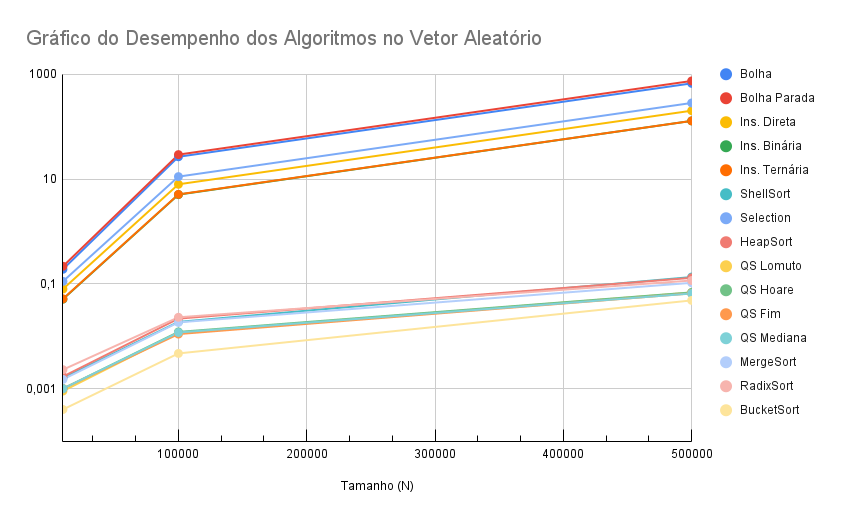
\includegraphics[width=\textwidth]{grafico_aleatorio.png}
\caption{Tempo de execução dos algoritmos em função do tamanho do vetor (entrada aleatória).}
\label{fig:grafico-aleatorio}
\end{figure}

\subsection{Análise em Vetores de Ordem Crescente}

\begin{table}[H]
\centering
\caption{Desempenho dos algoritmos – Entrada Crescente}
\label{tab:aleatoria}

\renewcommand{\arraystretch}{1.45} 
\LARGE

\resizebox{\textwidth}{!}{
\begin{tabular}{|l|c|c|c|c|c|c|c|c|c|}
\hline
\textbf{Algoritmo} 
& \multicolumn{3}{c|}{\textbf{10.000}} 
& \multicolumn{3}{c|}{\textbf{100.000}} 
& \multicolumn{3}{c|}{\textbf{500.000}} \\
\cline{2-10}

& \textbf{Comp.} & \textbf{Trocas} & \textbf{Tempo (s)}
& \textbf{Comp.} & \textbf{Trocas} & \textbf{Tempo (s)}
& \textbf{Comp.} & \textbf{Trocas} & \textbf{Tempo (s)} \\
\hline

Bolha & 49995000 & 0 & 0.103526 & 4999950000 & 0 & 10.384914 & 124999750000 & 0 & 261.569666 \\ \hline
Bolha c/ Critério de Parada & 9999 & 0 & 0.000025 & 99999 & 0 & 0.000232 & 499999 & 0 & 0.001183 \\ \hline
Inserção Direta & 9999 & 0 & 0.000031 & 99999 & 0 & 0.000293 & 499999 & 0 & 0.001822 \\ \hline
Inserção Binária & 113631 & 0 & 0.000712 & 1468946 & 0 & 0.004553 & 8475732 & 0 & 0.026182 \\ \hline
Inserção Ternária & 150486 & 0 & 0.000899 & 1934292 & 0 & 0.006134 & 11202852 & 0 & 0.036157 \\ \hline
Shell Sort & 75243 & 0 & 0.000501 & 967146 & 0 & 0.003441 & 5601426 & 0 & 0.019867 \\ \hline
Selection Sort & 50004999 & 0 & 0.110826 & 5000049999 & 0 & 11.081923 & 125000249999 & 0 & 279.900498 \\ \hline
Heap Sort & 381417 & 131957 & 0.001596 & 4813372 & 1650855 & 0.018077 & 27443486 & 9355701 & 0.100309 \\ \hline
Quick Sort Centro (Lomuto) & 113631 & 11808 & 0.000313 & 1468946 & 131070 & 0.003904 & 8475732 & 524286 & 0.021605 \\ \hline
Quick Sort Centro (Hoare) & 143615 & 0 & 0.000341 & 1768927 & 0 & 0.004131 & 9975711 & 0 & 0.022878 \\ \hline
Quick Sort Fim & 49995000 & 0 & 0.106133 & 4999950000 & 0 & 10.568094 & 124999750000 & 0 & 266.981449 \\ \hline
Quick Sort Mediana & 173612 & 0 & 0.000562 & 2068924 & 0 & 0.004629 & 11475708 & 0 & 0.025320 \\ \hline
Merge Sort & 64608 & 133616 & 0.001203 & 815024 & 1668928 & 0.011289 & 4692496 & 9475712 & 0.073830 \\ \hline
Radix Sort & 0 & 50000 & 0.001314 & 0 & 600000 & 0.011196 & 0 & 3000000 & 0.056684 \\ \hline
Bucket Sort & 0 & 10000 & 0.000358 & 0 & 100000 & 0.003478 & 0 & 500000 & 0.041502 \\ \hline

\end{tabular}
}
\end{table}

A partir da tabela de desempenho para entrada crescente, observa-se que vários algoritmos apresentam comportamento significativamente melhor em comparação ao caso aleatório. Algoritmos como Bolha com parada, Inserção Direta e Inserção Binária/Ternária realizaram um número muito reduzido de comparações e praticamente nenhuma troca, refletindo tempos de execução extremamente baixos mesmo para vetores de 500.000 elementos. Isso ocorre porque esses algoritmos se beneficiam diretamente do fato de o vetor já estar ordenado, explorando a melhor situação possível prevista em suas análises teóricas.

Em contrapartida, algoritmos que não se adaptam à ordem inicial dos dados, como Selection Sort e o Bolha tradicional, continuam apresentando comportamento quadrático. Mesmo sem realizar trocas, esses algoritmos percorrem todo o vetor em busca do menor elemento ou para verificar ordenação, resultando em um número muito elevado de comparações e tempos de execução altos para entradas grandes. O mesmo efeito é observado no Quick Sort com pivô no fim, que sofre forte degradação em vetores crescentes, aproximando-se do pior caso O(n²), o que explica os tempos elevados registrados. Deve-se enfatizar que o código do Quick Sort Fim teve que ser alterado pois no cenário de 500.000 elementos em ordem crescente, sua recursão exigiu muita memória e na execução deu falha de segmentação.

Por outro lado, algoritmos de complexidade O(n log n), como Heap Sort, Merge Sort e as variações mais robustas do Quick Sort (especialmente com mediana ou pivô central), mantiveram desempenho eficiente e estável. Além disso, os algoritmos não comparativos, como Radix Sort e Bucket Sort, apresentaram tempos baixos e crescimento linear, independentemente da ordenação inicial. De modo geral, os resultados confirmam que entradas crescentes favorecem algoritmos adaptativos, enquanto reforçam a importância de boas estratégias de pivô e do uso de algoritmos mais eficientes para evitar degradações severas de desempenho.

\begin{figure}[H]
\centering
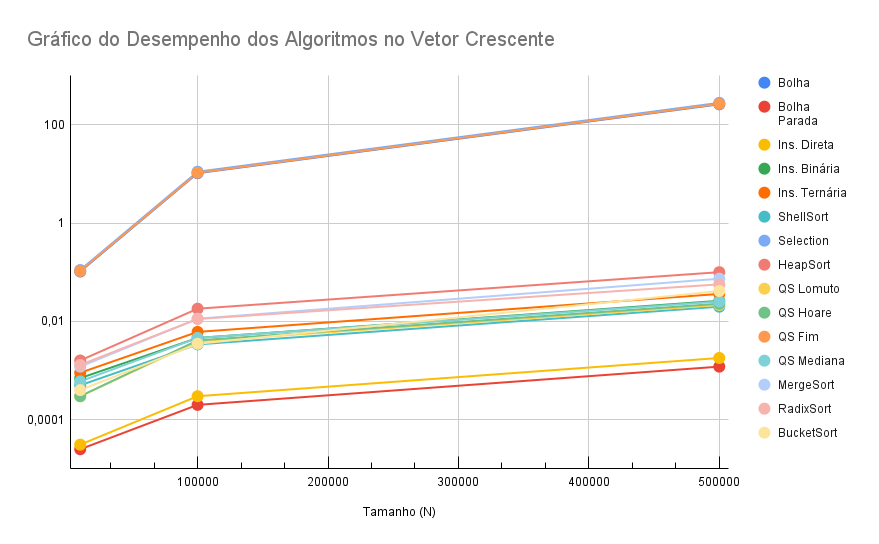
\includegraphics[width=\textwidth]{grafico_crescente.png}
\caption{Tempo de execução dos algoritmos em função do tamanho do vetor (entrada crescente).}
\label{fig:grafico-crescente}
\end{figure}

\subsection{Análise em Vetores de Ordem Decrescente}

\begin{table}[H]
\centering
\caption{Desempenho dos algoritmos – Entrada Decrescente}
\label{tab:aleatoria}

\renewcommand{\arraystretch}{1.45} 
\LARGE

\resizebox{\textwidth}{!}{
\begin{tabular}{|l|c|c|c|c|c|c|c|c|c|}
\hline
\textbf{Algoritmo} 
& \multicolumn{3}{c|}{\textbf{10.000}} 
& \multicolumn{3}{c|}{\textbf{100.000}} 
& \multicolumn{3}{c|}{\textbf{500.000}} \\
\cline{2-10}

& \textbf{Comp.} & \textbf{Trocas} & \textbf{Tempo (s)}
& \textbf{Comp.} & \textbf{Trocas} & \textbf{Tempo (s)}
& \textbf{Comp.} & \textbf{Trocas} & \textbf{Tempo (s)} \\
\hline

Bolha & 49995000 & 49995000 & 0.230836 & 4999950000 & 4999950000 & 23.082173 & 124999750000 & 124999750000 & 580.236855 \\ \hline
Bolha c/ Critério de Parada & 49995000 & 49995000 & 0.244767 & 4999950000 & 4999950000 & 24.592141 & 124999750000 & 124999750000 & 615.809150 \\ \hline
Inserção Direta & 49995000 & 49995000 & 0.158200 & 4999950000 & 4999950000 & 15.922399 & 124999750000 & 124999750000 & 399.273143 \\ \hline
Inserção Binária & 123617 & 49995000 & 0.102209 & 1568929 & 4999950000 & 10.078137 & 8975713 & 124999750000 & 252.024385 \\ \hline
Inserção Ternária & 80159 & 49995000 & 0.100868 & 1011427 & 4999950000 & 10.239445 & 5734280 & 124999750000 & 253.631080 \\ \hline
Shell Sort & 120190 & 53704 & 0.000447 & 1533494 & 619654 & 0.005304 & 8622570 & 3451804 & 0.030303 \\ \hline
Selection Sort & 50004999 & 5000 & 0.112182 & 5000049999 & 50000 & 11.228355 & 125000249999 & 250000 & 281.507566 \\ \hline
Heap Sort & 348379 & 116697 & 0.001406 & 4474075 & 1497435 & 0.017096 & 25896448 & 8668451 & 0.096554 \\ \hline
Quick Sort Centro (Lomuto) & 117534 & 63490 & 0.000492 & 1513481 & 795726 & 0.005860 & 8699870 & 4585604 & 0.033126 \\ \hline
Quick Sort Centro (Hoare) & 143616 & 5000 & 0.000349 & 1768928 & 50000 & 0.004236 & 9975712 & 250000 & 0.023092 \\ \hline
Quick Sort Fim & 49995000 & 5000 & 0.106889 & 4999950000 & 50000 & 10.311209 & 124999750000 & 250000 & 258.823363 \\ \hline
Quick Sort Mediana & 173613 & 5002 & 0.000416 & 2068925 & 50002 & 0.005350 & 11475709 & 250002 & 0.025877 \\ \hline
Merge Sort & 69008 & 133616 & 0.001251 & 853904 & 1668928 & 0.011206 & 4783216 & 9475712 & 0.063108 \\ \hline
Radix Sort &0 & 50000 & 0.001321 & 0 & 600000 & 0.011230 & 0 & 3000000 & 0.057642 \\ \hline
Bucket Sort & 0 & 10000 & 0.000831 & 0 & 100000 & 0.003537 & 0 & 500000 & 0.022287 \\ \hline

\end{tabular}
}
\end{table}

A partir da tabela de desempenho para entrada decrescente, observa-se que esse cenário representa um dos casos mais desfavoráveis para diversos algoritmos clássicos. Os algoritmos Bolha, Bolha com parada e Inserção Direta apresentam números extremamente elevados de comparações e trocas, o que resulta em tempos de execução muito altos à medida que o tamanho do vetor cresce. Isso ocorre porque, em um vetor decrescente, esses métodos precisam efetivamente reorganizar todos os elementos, caracterizando o pior caso O(n²), o que se reflete claramente nos resultados obtidos.

No caso dos algoritmos baseados em Quick Sort, o impacto da escolha do pivô torna-se evidente. A versão com pivô no fim sofre forte degradação, apresentando desempenho semelhante ao dos algoritmos quadráticos, com tempos elevados para entradas maiores. Em contrapartida, as versões com pivô central (Lomuto e Hoare) e com mediana mantêm um número de comparações e trocas significativamente menor, resultando em tempos muito inferiores. Isso confirma que estratégias mais robustas de escolha de pivô reduzem a probabilidade de cair no pior caso, mesmo em entradas altamente desfavoráveis como a decrescente.

Por outro lado, algoritmos com complexidade O(n log n), como Heap Sort e Merge Sort, demonstram maior estabilidade frente à ordenação inicial dos dados, apresentando crescimento controlado do tempo de execução. Além disso, os algoritmos não comparativos, Radix Sort e Bucket Sort, mantêm desempenho eficiente e praticamente linear, independentemente da ordem de entrada. De forma geral, os resultados evidenciam que a entrada decrescente penaliza fortemente algoritmos quadráticos e versões ingênuas do Quick Sort, reforçando a importância da escolha adequada do algoritmo conforme as características do conjunto de dados.

\begin{figure}[H]
\centering
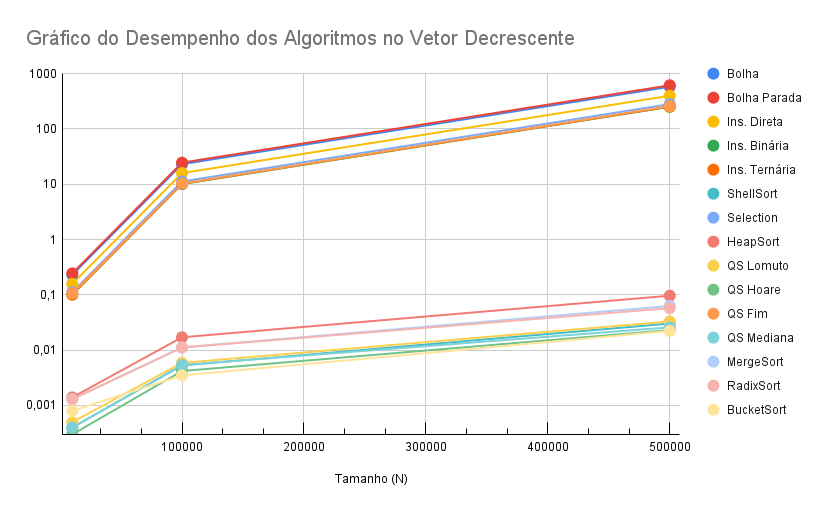
\includegraphics[width=\textwidth]{grafico_decrescente.png}
\caption{Tempo de execução dos algoritmos em função do tamanho do vetor (entrada decrescente).}
\label{fig:grafico-decrescente}
\end{figure}

% ---------------- CONCLUSÃO ----------------
\section{Conclusão}

De modo geral, os resultados obtidos ao longo deste trabalho evidenciam de forma clara como o desempenho dos algoritmos de ordenação está diretamente relacionado tanto à sua complexidade assintótica quanto à ordem inicial dos dados de entrada. A análise comparativa entre vetores aleatórios, crescentes e decrescentes permitiu observar, na prática, conceitos frequentemente discutidos apenas de forma teórica, como pior caso, melhor caso e caso médio. Em especial, algoritmos de complexidade quadrática, como Bolha, Bolha com critério de parada, Selection Sort e Inserção Direta, mostraram-se inviáveis para grandes volumes de dados nos cenários aleatório e decrescente. Embora o critério de parada reduza o custo em entradas já ordenadas, seu impacto é mínimo quando os dados se encontram desorganizados, mantendo o elevado número de comparações e o alto tempo de execução.

Os algoritmos baseados em Quick Sort demonstraram comportamento fortemente dependente da estratégia de escolha do pivô. Versões mais simples, como o pivô no fim, sofreram degradação significativa em entradas ordenadas ou inversamente ordenadas, enquanto abordagens mais robustas, como pivô central e mediana, mantiveram desempenho próximo ao esperado O(n log n). Isso reforça a importância de decisões de implementação aparentemente simples, que podem impactar drasticamente o desempenho prático do algoritmo.

Algoritmos como Merge Sort e Heap Sort apresentaram desempenho estável em todos os cenários analisados, confirmando sua previsibilidade e robustez independentemente da distribuição dos dados. Já os algoritmos não comparativos, como Radix Sort e Bucket Sort, destacaram-se pelos baixos tempos de execução e crescimento praticamente linear, desde que as condições de aplicação fossem adequadas. Esses resultados mostram que, quando aplicáveis, tais algoritmos podem ser significativamente mais eficientes do que métodos baseados em comparação.

Por fim, este estudo reforça que não existe um algoritmo de ordenação universalmente superior para todos os casos. A escolha adequada depende do tamanho do vetor, da distribuição dos dados, das restrições de memória e do custo das operações envolvidas. Assim, a compreensão tanto teórica quanto prática do comportamento dos algoritmos torna-se essencial para a tomada de decisões eficientes em problemas reais, evidenciando a relevância do estudo aprofundado de algoritmos e estruturas de dados na área da computação.

\bibliographystyle{apalike}
\bibliography{referencias}

\end{document}


